\documentclass[11pt, a4paper, doubleside]{Thesis}
\graphicspath{{./Pictures/}} % Specifies the directory where pictures are stored
\usepackage[utf8]{inputenc}
\setlength\parindent{24pt}

\usepackage{arydshln}%dibujar lineas verticales y horizontales
\usepackage{mathtools}
\usepackage{graphicx}
\usepackage[T1]{fontenc}
\usepackage{amssymb,graphicx}
\usepackage[utf8]{inputenc}
\usepackage{mathtools}
\usepackage{MnSymbol}
\usepackage{stmaryrd}
\usepackage{amsfonts}
\usepackage{amsmath}
\usepackage{amssymb}
\usepackage[all]{xy}

\usepackage[USenglish]{babel}

\newtheorem{theorem}{Theorem}[section]
\newtheorem{coro}{Corollary}[theorem]
\newtheorem{propo}{Proposition}[theorem]
\newtheorem{lemma}{Lemma}[theorem]
\newtheorem{defini}{Definition}[theorem]
\newtheorem{conje}[theorem]{Conjecture}
\newtheorem{prob}[theorem]{Problem}

\newtheorem{ejemp}[theorem]{Example}
\newtheorem{cond}[theorem]{Condition}
\newtheorem{nota}[theorem]{Note}
\newtheorem{notation}[theorem]{Notation}
\newtheorem{conv}[theorem]{Convention}

\newcommand{\E}{\mathbb{E}}
\newcommand{\F}{\mathcal{F}}
\newcommand{\R}{\mathbb{R}}
\newcommand{\Q}{\mathbb{Q}}
\newcommand{\N}{\mathbb{N}}
\newcommand{\Z}{\mathbb{Z}}
\renewcommand{\P}{\mathbb{P}}
\renewcommand{\G}{\mathcal{G}}
\renewcommand{\S}{\mathbb{S}}



\newenvironment{cajita}
    {\begin{center}
    \begin{tabular}{|p{0.9\textwidth}|}
    \hline\\
    }
    { 
    \\\\\hline
    \end{tabular} 
    \end{center}
    }  
    

\usepackage[table]{xcolor}
\definecolor{Blue}{HTML}{006699}
\definecolor{Green}{HTML}{4F9C45}

\providecommand{\abs}[1]{\lvert#1\rvert}

\title{\ttitle} % Defines the thesis title - don't touch this

\begin{document}

\frontmatter % Use roman page numbering style (i, ii, iii, iv...) for the pre-content pages

\setstretch{1.3} % Line spacing of 1.3

% Define the page headers using the FancyHdr package and set up for one-sided printing
\fancyhead{} % Clears all page headers and footers
\rhead{\thepage} % Sets the right side header to show the page number
\lhead{} % Clears the left side page header

\pagestyle{fancy} % Finally, use the "fancy" page style to implement the FancyHdr headers

\newcommand{\HRule}{\rule{\linewidth}{0.5mm}} % New command to make the lines in the title page

% PDF meta-data
\hypersetup{pdftitle={\ttitle}}
\hypersetup{pdfsubject=\subjectname}
\hypersetup{pdfauthor=\authornames}
\hypersetup{pdfkeywords=\keywordnames}

%----------------------------------------------------------------------------------------
%	TITLE PAGE
%----------------------------------------------------------------------------------------

%\begin{titlepage}
%\phantom{Hola}
%\end{titlepage}
%\clearpage

%----------------------------------------------------------------------------------------
%	Frase conmovedora
%----------------------------------------------------------------------------------------

%\pagestyle{empty} % No headers or footers for the following pages

%\null\vfill % Add some space to move the quote down the page a bit
%\begin{flushright}
%\textit{
%Don’t only practice your art, but force your way into its secrets, for it and knowledge can raise men to the divine.
%}
%\end{flushright}

%\begin{flushright}
%Celso Chávez Mendoza (fragmento).
%\end{flushright}

%\vfill\vfill\vfill\vfill\vfill\vfill\null % Add some space at the bottom to position the quote just right
%\clearpage


%----------------------------------------------------------------------------------------
%	ACKNOWLEDGEMENTS
%----------------------------------------------------------------------------------------

%\setstretch{1.3} % Reset the line-spacing to 1.3 for body text (if it has changed)

%\acknowledgements{\addtocontents{toc}{\vspace{1em}} % Add a gap in the Contents, for aesthetics
%}
%\clearpage % Start a new page

%----------------------------------------------------------------------------------------
%	LIST OF CONTENTS/FIGURES/TABLES PAGES
%----------------------------------------------------------------------------------------

\pagestyle{fancy} % The page style headers have been "empty" all this time, now use the "fancy" headers as defined before to bring them back

\lhead{\emph{Indice}} % Set the left side page header to "Contents"
\tableofcontents % Write out the Table of Contents

%\lhead{\emph{List of Figures}} % Set the left side page header to "List of Figures"
%\listoffigures % Write out the List of Figures

%\lhead{\emph{List of Tables}} % Set the left side page header to "List of Tables"
%\listoftables % Write out the List of Tables

%----------------------------------------------------------------------------------------
%	RESUMEN PAGE
%----------------------------------------------------------------------------------------

%\begin{Resumen}


%\vspace{5cm}

%\textit{Palabras clave:} 
%\end{Resumen}

%----------------------------------------------------------------------------------------
%	ABSTRACT PAGE
%----------------------------------------------------------------------------------------

\begin{abstract}

%In this work we propose the use of the Radó graph and the Erdös Rényi model for random graphs to study a rigidity phenomenon in graphs called rigid expansions. We review the motivation to stud
rg
%The goal is to do it in the curve graph associated to a surface $S$, we will show the conditions under which is possible to do it in a simple probabilistic model.

\end{abstract}

%----------------------------------------------------------------------------------------
%	ABBREVIATIONS
%----------------------------------------------------------------------------------------

%\clearpage % Start a new page

%\setstretch{1.5} % Set the line spacing to 1.5, this makes the following tables easier to read

%\lhead{\emph{Abbreviations}} % Set the left side page header to "Abbreviations"

%\listofsymbols{ll} % Include a list of Abbreviations (a table of two columns)
%{
%\textbf{LAH} & \textbf{L}ist \textbf{A}bbreviations \textbf{H}ere \\
%\textbf{Acronym} & \textbf{W}hat (it) \textbf{S}tands \textbf{F}or \\
%}

%----------------------------------------------------------------------------------------
%	SYMBOLS
%----------------------------------------------------------------------------------------

\clearpage % Start a new page

\lhead{\emph{Symbols}} % Set the left side page header to "Symbols"

%\listofnomenclature{ll}{ % Include a list of Symbols (a three column table)
%$K\RFD L$ & Retracto por deformación fuerte. \\
%$J^{n}$& $Cl(\partial I^{n+1} - I^{n})$ (Caja sin tapa inferior).\\
%$L < K$& $L$ es un subcomplejo de $K$.\\
%$K\CElem L$ & $K$ colapsa elementalmente a $L$. \\
%$K\EElem L$ & $K$ se expande elementalmente a $L$. \\
%$K\searrow L$ & Existe una sucesión finita de colapsos elementales de $K$ a $L.$
%\\
%$K\nearrow L$ & Existe una sucesión finita de expansiones elementales de $K$ a $L.$
%\\
%$K\SimpHomEq L$ & Existe una sucesión finita de colapsos y expansiones elementales de $K$ a $L.$
%}

%----------------------------------------------------------------------------------------
%	DEDICATION
%----------------------------------------------------------------------------------------

\setstretch{1.3} % Return the line spacing back to 1.3

\pagestyle{empty} % Page style needs to be empty for this page

\dedicatory{} % Dedication text

\addtocontents{toc}{\vspace{2em}} % Add a gap in the Contents, for aesthetics



%----------------------------------------------------------------------------------------
%	THESIS CONTENT - CHAPTERS
%----------------------------------------------------------------------------------------

\mainmatter % Begin numeric (1,2,3...) page numbering

\pagestyle{fancy} % Return the page headers back to the "fancy" style

% Include the chapters of the thesis as separate files from the Chapters folder
% Uncomment the lines as you write the chapters
% Introducción
\chapter*{Introduction} % Main chapter title

\label{Intro} % For referencing the chapter elsewhere, use \ref{Chapter1} 

\lhead{\emph{Introduction}} % This is for the header on each page - perhaps a shortened title

%----------------------------------------------------------------------------------------
%----------------------------------------------------------------------------------------
%	INTRODUCTION
%----------------------------------------------------------------------------------------

The curve graph $\Gamma(S)$ associated to a surface $S$ appears naturally in the study of $Mod(S)$, the mapping class group of $S$, which is a central subject in contemporary mathematical research. We are interested in a rigidity concept of this graph; in general, the idea behind rigidity phenomena is to describe morphisms among objects using their structure.

The folkloric version of rigidity in the $Mod(S)$ context is that if we consider $X$ and $Y$, under suitable conditions, then every homomorphism $Mod(X) \to Mod(Y)$ will be induced by a manipulation of the underlying surfaces.

Ivanov sketched in \cite[Ivanov, 1997]{metaconjecture} the proof that every automorphism of $C(S)$ (the flag complex of $\Gamma(S)$), is induced by a self-homeomorphism of $S$. This argument is the favorite in the literature due to its simplicity and resemblance to proofs of other rigidity results.

A research line lead by Aramayona and Leininger propose the idea of \textit{rigid sets}, which can be interpreted as a subset \textit{that allows to extend a local notion of rigidity to global one}. In the aim of finding large rigid sets, in \cite[Aramayona, Leininger - 16]{exhaustionByRigidSets} there's the proof of the existence of an increasing sequence of finite rigid sets that exhaust the curve graph. For this, they proposed a method called \textbf{rigid expansions}.

Rigidity in graphs is, regardless of its interpretation in the curve graph, an interesting phenomenon by it self. Due to the discrete nature of rigid expansions is reasonable to seek for a probabilistic approach; our goal is to address this particular path.

We want to answer the rather vague question: \textit{How \textbf{common} is rigidity in graphs}, specifically by answering \textit{how rigid expansions \textbf{usually} behave}. Also, the aim of the thesis is to review the feasibility of \textit{studying the curve complex of a surface in a probabilistic point of view.}

To give formal meaning to words like "common" or "usually" in rigidity's panorama, is required the use of \textit{simple} probabilistic models which allows to study such complex phenomenon. Then, we will analyze the conditions under which these models can fit the known properties of the curve graph.

In chapter one, we motivate the study of the curve graph and review the most important properties of it. Then, we will introduce rigidity from the graph theory context.

In the second chapter, we propose the study of rigidity in the stochastic context through the Radó graph and the Erdös-Rényi model. In the aim to study the curve graph of a surface with a simple model, we justify that the genus of the surface cannot be finite. Thus, we end up with an asymptotic probabilistic analogue to the result due to Bering and Gaster, which asserts that the Radó graph embeds into the curve graph $C(S)$ of a surface $S$ if and only if $S$ has infinite genus.

Finally, we made a computational implementation of the algorithm to do rigid expansions. With the corresponding optimizations that the method require, we were able to take a closer look to rigidity phenomena.
% Chapter 1

\chapter{The curve graph of a surface} % Main chapter title

\label{Chapter1} % For referencing the chapter elsewhere, use \ref{Chapter1} 

\lhead{Chapter 1. \emph{The curve graph of a surface}} % This is for the header on each page - perhaps a shortened title

%----------------------------------------------------------------------------------------

The study of surfaces in a strictly topological viewpoint has led us to forget significant information about them. A way to revert this is to attach a group to it, the \textbf{mapping class group} of the surface. It is denoted by $Mod(S)$ and encodes the \textit{symmetries} of the surface. This group is defined as the set of isotopy classes of orientation-preserving homeomorphisms of $S$. In the first section of this chapter we give the formal definition of this group and establish the very important role of this concept in Mathematics. 

The \textbf{curve complex} of the surface, denoted by $C(S)$ appears naturally in the study of $Mod(S)$. It is a simplicial complex that encodes intersection patterns of simple closed curves in $S$. We focus part of the discussion in the relationship between the algebraic structure of $Mod(S)$ and the combinatorial topology of $S$.

Many of the progress in understanding $Mod(S)$ has been possible by a well-known analogy among two very important classes of groups: arithmetic groups and mapping class groups. In this parallelism panorama arises the desire for an equivalent result to the Margulis Superrigidity for mapping class groups.

In the last section of this chapter we settle the bases to understand rigidity within a Graph theory context. An approach called \textit{rigid expansions}, see \cite[Aramayona, Leininger 16]{finiteRigidSetsJA} and \cite[Hernandez 19]{exhaustionCurveGraph}, allows us to build up subgraphs preserving the rigidity property and is compatible with stochastic tools.
 
Many results and definitions in this chapter where extracted from \cite[Farb]{Farb}. They are quite popular and equivalents can easily be found in the literature, however they are written here to establish nomenclature. Familiarity with basic concepts is assumed.

\section{Mapping class group of a surface}

We have the following fundamental, well-known result about surfaces.

\begin{theorem}[Classification of surfaces]\label{CST}
Any closed, connected, orientable surface is homeomorphic to the connect sum of a 2-dimensional sphere with $g \geq 0$ tori. Any compact, connected, orientable surface is obtained from a closed surface by removing $b \geq 0 $ open disks with disjoint closures. Even more, the set of homeomorphism types of compact surfaces is in bijective correspondence with the set $\{ (g, b) : g, b \geq 0\}$.
\end{theorem}

We are so familiarized with this result that we usually forget what it is saying. It seems like, in the eyes of a topologist, there is nothing much interesting about surfaces, but this is because we are forgetting all the geometric information about them. $Mod(S)$ helps to recover this data, the magic happens when this group acts on the \textbf{Teichmüller space} of $S$, that is the space of hyperbolic metrics on $S$ up to isotopy. A central result is that this action is properly discontinuous and the quotient space $M(S) = Teich(S)/ Mod(S)$ is the \textbf{moduli space of Riemannian surfaces homeomorphic to $S$}. The space $M(S)$ is a essential object in mathematics and the group $Mod(S)$ encodes most of the topological features of $M(S)$.

$Mod(S)$, $Teich(S)$, and $M(S)$ can be found in a lot of different contexts in mathematics: hyperbolic geometry, algebraic geometry, combinatorial group theory, symplectic geometry, 3-manifold theory, dynamics and so on. The algebraic structure of $Mod(S)$, the geometry of $Teich(S)$, and the topology of $M(S)$ are just the strands which are used to weave the rich tapestry of the nature of the surface.

Before we continue, let's establish some nomenclature. The $g$ in \ref{CST} is called the \textit{genus} of the surface and the $b$ is the number of \textit{boundary components}. One way to obtain a non-compact surface from a compact one is to remove $m$ points from the interior of it; in this case, we say that the resulting surface has $m$ punctures. For now on, unless otherwise specified, we will be thinking in compact, connected, oriented surfaces that are possibly punctured (in this case they ceases to be compact). Therefore, we can specify the surfaces by the triplet $(g, b, m)$. We will denote by $S_{g,m}$ a surface of genus $g$ with $m$ punctures and empty boundary; such a surface is homeomorphic to the interior of a compact surface with $m$ boundary components. Also, for a closed surface of genus $g$, we will abbreviate $S_{g,0}$ as $S_{g}$ and $\partial S$ denote the (possibly disconnected) boundary of $S$.

There are a number of definitions for the mapping class group of a surface. We will be working with the following:

\begin{defini}
Let $S$ be a surface, the \textbf{mapping class group} of $S$, denoted by $Mod(S)$ is the following quotient:
$$Mod(S)=Homeo^{+}(S)/Homeo_{0}(S)$$
where $Homeo^{+}(S)$ is the group of orientation-preserving, homeomorphisms of $S$, that are the identity on the boundary, this group can be endowed with the compact-open topology. $Homeo_{0}(S)$ is the subgroup formed by homeomorphisms of $S$ which are isotopic to the identity, i.e. the connected component of the identity with this topology.
\end{defini}

We could consider diffeomorphisms instead of homeomorphisms, or homotopy classes instead of isotopy classes; this will result in isomorphic groups, see \cite[Farb, p.~41]{Farb} for details in why we can do this. Summarizing, we can find the following variations in the definition of $Mod(S)$:

\centerline{\begin{tabular}{ rcl }
$Mod(S)$ & $=$ & $\pi_{0}(Homeo^{+}(S, \partial S))$\\
 & $\approx$ & $Homeo^{+}(S,\partial S)/\textit{homotopy}$\\
 & $\approx$ & $\pi_{0} (\textit{Diff}^{+}(S,\partial S))$\\
\end{tabular}}

where $\textit{Diff}^{+}(S, \partial S)$ is the group of orientation-preserving diffeomorphisms of $S$ that are the identity on the boundary. It can be taken to be either smooth homotopy relative to the boundary or smooth isotopy relative to the boundary.

A lot of work had been made to describe the types of elements in $Mod(S)$. Thanks to the Thurston's classification theorem there is a characterization of the homeomorphisms of a compact orientable surface. This classification is useful to describe the curve graph which will be analyzed in the next section.

\subsection{Nielsen–Thurston classification}
Given a homeomorphism $f: S \to  S$, there is a map $g$ isotopic to $f$ such that at least one of the following statements holds:

\begin{itemize}
\item $g$ is periodic, i.e. some power of $g$ is the identity;
\item $g$ preserves some finite union of disjoint simple closed curves on $S$ (in this case, g is called reducible); or
\item $g$ is pseudo-Anosov.
\end{itemize}

The definition of a \textbf{pseudo-Anosov map} relies on the notion of a measured foliation, a geometric structure on $S$. It consists of a singular foliation and a measure in the transverse direction (i.e. that is constant in transverse arches). For the full definition of pseudo-Anosov elements and the proof of this theorem we can refer to \cite[Farb, ch.~13]{Farb}.

The study of mapping class groups is a wide and challenging area. It is outside of the interests of this thesis to review the details and repercussions of this vastly field. Yet, there are a number of known properties of $Mod(S)$ that it would be nice to have in mind in further work, although different tools might be required.

\begin{itemize}
\item Finitely generated and presented
\item It has a subgroup of finite index which doesn't have torsion.
\item $Mod(S_{g,m}) \cong Out(\pi_{1}(S_{g,m}))$
\item $H_{1}(Mod(S_{g,m}), \Z) = 1$ when $(g\geq3, m=0)$
\end{itemize}

\section{Curve graph}

\subsection{Simple closed curves}

\begin{defini}
A \textbf{closed curve} in a surface $S$ is a continuous map $\S^{1}\to S$, is called \textbf{simple} if the map is injective. We will usually identify a closed curve with its image in $S$. A closed curve is called \textbf{essential} if it is not homotopic to a point, a puncture, or a boundary component.
\end{defini}
Among the adjectives that a curve can acquired we have the following:
\begin{itemize}
    \item $\alpha$ is \textbf{separating}, if $S-\alpha$ has two components, otherwise it is called \textbf{non separating}.
    \item It is called \textbf{essential} if no component of $S- \alpha$ is a disk.
    \item It is \textbf{non-peripheral} if no component of $S - \alpha$ is an annulus. 
\end{itemize}

We are interested in \textbf{essential} and \textbf{non-peripherial} curves, they will be assumed in this sense, unless otherwise specified.

The idea behind the construction of the curve graph is to stratify the set of homotopy classes of curves on a surface. For this to make sense we define the \textbf{geometric intersection number} between free homotopy classes $a$ and $b$ of simple closed curves in a surface $S$. This is defined to be the minimal number of intersection points between a representative curve in the class $a$ and a representative curve in the class $b$:
$$i(a,b) = min \{ |\alpha \cap \beta| : \alpha \in a, \beta \in b \}$$
It is convenient to adopt a slight abuse of notation by writing $i(\alpha, \beta)$ for the intersection number between the homotopy classes of simple closed curves $\alpha$ and $\beta$. It is useful to think that this number can be calculate by finding representatives $\alpha$ and $\beta$ that achieve the minimal intersection in their homotopy classes, so that $i(a, b) = |\alpha \cap \beta|$ (when this is the case, we say that $\alpha$ and $\beta$ are in minimal position). Although the geometric intersection number is a useful and intuitive invariant it is not always easy to compute, whenever this is the case we can appeal to the algebraic intersection number. For a further discussion of this see \cite[Farb]{Farb}

\subsection{The curve graph}

\begin{defini}
The \textbf{curve graph} $\Gamma(S)$ of a surface $S$ is constructed by the following data:
\begin{itemize}
\item \textbf{Vertices}. There's a vertex in $\Gamma(S)$ for every isotopy class of essential closed curves in $S$.
\item \textbf{Edges}. There's an edge between the corresponding vertices of isotopy classes $a$ and $b$ whenever $i(a,b)=0$.
\end{itemize}
\end{defini}

\begin{defini}
The \textbf{curve complex of the surface}, $C(S)$ is defined to be the flag complex of the curve graph just defined.
\end{defini}

\section{Properties of the curve graph}
The goal of this section is to enumerate known properties of the curve graph, we use this to establish the appropriate parameters in a probabilistic model. Notice that the construction of the curve complex is completely determined by the curve graph, hence the probabilistic models can work in the same sense. Lets keep in mind the following exceptional cases; they are responsible for the conditions stated in the hypothesis of the following theorems for $g$ and $n$. For $ S^2, S_{0,1}, S _{0,2}, S_{0,3} $ the curve graph is empty and for  $ T^{2} $, $ S_{1,1}$ and $ S_{0,4}$ is a countable disjoint union of points.

\subsection{Cardinality of the number of vertices}
\begin{theorem}
If $g\geq 1$ or $n\geq 4$ then the set of vertices in $\Gamma(S_{g,n})$ is countably infinite.
\end{theorem}

It is well known that for $T^{2}$ there is an explicit identification for the isotopy classes of essential curves with the rational numbers. In this case there aren't disjoint curves, the following figure can help to convince us of this fact.
\vspace{0.5cm}
\begin{figure}[h!]
	\centering
	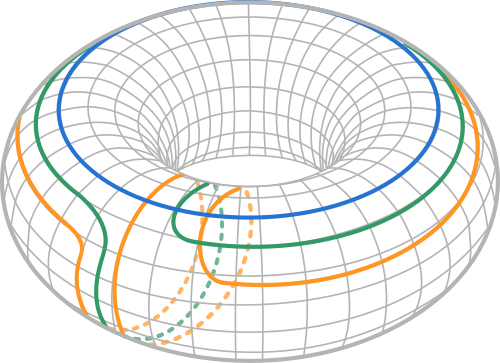
\includegraphics[scale=1]{Figures/Torus.png}
	\caption{$T^{2}$ with representatives of typical elements of curves}
\end{figure}

This identification can be seen as the induction basis. The induction step over $g$ comes from splitting the surface, by induction hypotheses none of the resulting surfaces can have a non-countable number of classes of curves.

\subsection{Connectivity}
\begin{theorem}
If $3g+n\geq 5$, then $\Gamma(S_{g,n})$ is connected.
\end{theorem}

To proof this theorem we can show that, for any two isotopy classes $a$ and $b$ of simple closed curves in $S_{g,n}$ exists a sequence of isotopy classes
$$a=c_{1},\dots,c_{k}=b$$
where $i(c_{i},c_{i+1})=0$, this can be done proceeding by induction over $i(a,b)$. The full proof of this theorem can be found in \cite[Farb, p.~93]{Farb} 

\subsection{Locally infinite}
\begin{theorem}
If $3g+m\geq 5$, then $\Gamma(S_{g,n})$ is locally infinite.
\end{theorem}
The idea behind the proof is that given any $\alpha \in \Gamma(S)$ we can construct a family of isotopy classes of curves which are disjoint to $\alpha$. The following picture gives us an intuitive idea on how to do this whenever there are enough holes.
\vspace{0.5cm}
\begin{figure}[h!]
	\centering
	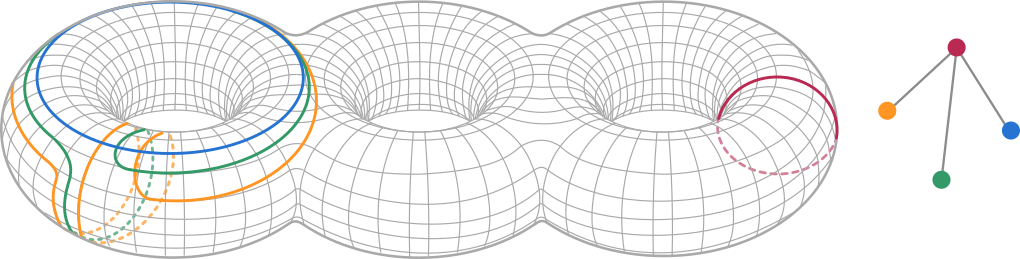
\includegraphics[scale=0.6]{Figures/Locally-infinite.png}
	\caption{$S_{3}$ with typical representative curves which exemplify the idea behind locally infinity property}
\end{figure}

For the complete argument, let $\alpha$ be any simple closed curve on $S$, the surface $S-\alpha$, obtained by cutting $S$ open along $\alpha$, contains at least one connected component of Euler characteristic at most $-2$ (guaranteed by the $3g+m\geq 5$ condition). Such component contains infinitely many distinct homotopy classes of simple closed curves disjoint from $\alpha$.

\subsection{Clique number}
A \textbf{clique} in a graph $G$ is a complete subgraph of $G$. The clique number $cl(G)$ of a graph $G$ is the maximum order of a clique of $G$.

\begin{theorem}
If $3g+n\geq 5$, then the clique number of $\Gamma(S_{g,m})$ is $3g - 3 + m$.
\end{theorem}

$3g-3+m$ is the number of curves in a pants decomposition of $S$, i.e. a maximal collection of disjoint, not freely homotopic, essential, simple closed curves which decompose $S$ into $2g-2+m$ open subsurfaces homeomorphic to a thrice punctures sphere. For a full proof of this well-known fact refer to \cite[Hatcher, Thurston 80]{Pants}

\vspace{0.5cm}
\begin{figure}[h!]
	\centering
	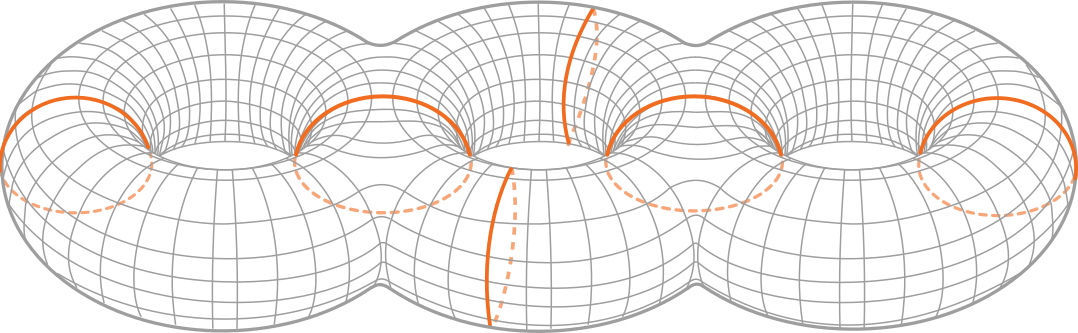
\includegraphics[scale=0.4]{Figures/Pantalones.png}
	\caption{Exemplification of a pants decomposition of a surface}
\end{figure}

\subsection{Infinite Diameter}
\begin{theorem}
If $3g+m\geq 5$ then $diam(\Gamma(S)) = \infty$
\end{theorem}

The proof for this theorem relies on the fact that for any pseudo-Anosov element $h \in Mod(S)$, any $\gamma \in V(\Gamma(S))$ and any $k\in \Z$
$$d_{C}\Big(h^{k}(\gamma), \gamma\Big) \geq c|k|$$
This provide the infinite diameter property. For details, refer to \cite[Masur, Minsky 99]{Masur}

The curve graph and the curve complex are fundamental tools in the study of the surfaces. There are a number of known properties of them that it would be nice to have in mind to improve probabilistic models in further work.

\begin{enumerate}
\item $C(S)$ is hyperbolic
\item In the infinite case $diam(\Gamma(S))= 2$
\item There's an isomorphism between $Mod(S)$ and $Aut(C(S))$, except when $(g,m) \in \{(1,2), (1,1), (2,0), (0,4)\}$
\end{enumerate}

\section{Rigidity in graphs}

The intention of this section is to track down the motivation of rigid expansions and give the required definitions.

As mention in the introduction of the chapter, rigidity appears in the mapping class group context in light of its comparison with arithmetic groups. In \cite[Aramayona, Souto 16]{rigidityJA} we can find a survey on the search of an analogue for the Margulis Superrigidity theorem. In this article, they provide three different perspectives: a Lie theoretical, a geometric and a folkloric one.

The Lie theoretic version states that every homomorphism $Mod(X) \to Mod(Y)$ is induced by a homomorphism between the associated groups of diffeomorphisms with compact support disjoint from the boundary $\textit{Diff}_{c}(X) \to \textit{Diff}_{c}(Y)$.

A direct formulation of geometric superrigidity cannot hold when the moduli space is endowed with any reasonable metric. However, there are ways to turn this around, saying that every (irreducible) homomorphism between mapping class groups induces a holomorphic map between the corresponding moduli spaces.

The folkloric version of Mostow and Margulis superrigidity claims that the only homomorphisms between lattices are the \textit{“obvious ones”}, in the $Mod(S)$ context this will mean that if we consider $X$ and $Y$, under suitable conditions, then every homomorphism $Mod(X) \to Mod(Y)$ will be induced by a manipulation of the underlying surfaces. 

A result due to Ivanov \cite[Ivanov 97]{celebratedIvanov}, Korkmaz \cite[Korkmaz 99]{celebratedKorkmaz} and Luo \cite[Luo 00]{celebratedLuo}, asserts that, excluding few well-understood cases, the curve complexes are simplicially rigid. This means that the group $Aut(C(S))$ of simplicial automorphisms of $C(S)$ is isomorphic to the extended mapping class group. This result is sometimes interpreted as a proof that \textbf{the automorphisms  of  the  curve  complex  are  all geometric}.

In the aim to generalize this result to broader types of simplicial self-maps, in \cite[Aramayona, Leininger 12]{finiteRigidSetsJA} was introduced the concept of \textbf{rigid sets} in the curve complex. Let $S$ be a surface different from $S_{1,2}$,  $Y \subset C(S)$ is called \textbf{rigid} if for every locally injective simplicial map $\Phi  : Y \to C(S)$ there exists $h \in Mod{\ast}(S)$ with $h|_{Y} = \Phi$, unique up to the pointwise stabilizer of $Y$ in $Mod^{\ast}(S)$.

Later in \cite[Aramayona, Leininger 16]{exhaustingCurveComplex} a method for enlarging rigid subgraphs is presented and the proof that for almost all surfaces of finite topological type, there exists an \textbf{increasing sequence of finite rigid sets} that exhaust the curve graph of which has trivial pointwise stabilizer in $Mod^{\ast}(S_{g},n)$.

In \cite[Hernández 19]{exhaustionCurveGraph} there is the proof of a similar result to Aramayona and Leininger's. The method,  called \textbf{rigid expansions}, allowed to obtain new results concerning edge-preserving maps. 

Losing the big picture that rigidity represents, we can land this vastly journey in the following graph theory definitions.

\begin{defini}
Let $\Gamma$ be a simplicial graph and $H<\Gamma$ a vertex-induced subgraph. A function $f:y\to \Gamma$ is \textbf{locally injective} if $f|_{star(v)}$ is injective for all $v \in V(y)$. 
\end{defini}

\begin{nota}
Remember, $star(v)$ is the vertex-induced subgraph with vertices $\{ v \} \cup N(v)$ ($v$ plus its neighborhood).
\end{nota}

\begin{defini}
$H<\Gamma$ is \textbf{rigid} if every locally injective function defined in $H$ can be extended to an automorphism of $\Gamma$. \end{defini}

A vertex $v \in V$ in a graph is called to be uniquely determined by $A\subset V(G)$, denoted $v=\langle A \rangle$, if $v$ is the unique common neighbor of every element of $B$, i.e.
$$ \{ v \} = \bigcap_{w\in B} lnk(w) $$
\begin{defini}
The first rigid expansion of $Y\subset \Gamma$, denoted by $Y^{1}$, is the vertex-induced subgraph whose vertices are
$$ V(Y) \cup \{ v\in V(\Gamma) :  \exists A \subset V(Y) \text{ where } v = \langle A \rangle  \}$$
We also define $Y^{0} = Y$ and, inductively, $Y^{k} = (Y^{k-1})^{1}$.
\end{defini}

Recalling that in Proposition 3.5 in \cite[Aramayona, Leininger 16]{finiteRigidSetsJA}, Aramayona and Leininger prove that if $Y \subset C(S)$ is a rigid set, then so is $Y^{r} $ for all $r \geq 0$. So this method in fact preserve the desired property.

It would be nice to have conditions which determine whether a subgraph is rigid or not. So far we know that there aren't non-trivial necessary conditions to check rigidity, i.e. other than connectivity there's not much else.

With this definitions we can proceed to settled a probabilistic model so that we can analyze the rigidity concept in graphs from a stochastic point of view. With the reviewed properties of the curve graph we can determine the feasibility of studying the curve graph through simple models.
% Chapter 2

\chapter{Rigidity in random graphs} % Main chapter title

\label{Chapter2} % For referencing the chapter elsewhere, use \ref{Chapter1} 

\lhead{Chapter 2. \emph{Rigidity in random graphs}} % This is for the header on each page - perhaps a shortened title

%----------------------------------------------------------------------------------------

The use of the probabilistic method in discrete mathematics has become a prominent idea in the area in recent times. It provide existence proofs where objects have certain desirable properties and it is not always easy to construct explicit examples. This has been just the beginning of the use of probabilistic tools in a deterministic context.

Complex topological spaces arise quite natural in a lot of scientific contexts. Probability theory implement different approaches to model those spaces; even in complex configurations, it can be possible by doing approximations, to study topological invariants. 

In this sense, stochastic topology can be thought as a tool for topology in the same sense as statistical mechanics is used to study a macroscopic physical system when the classical mechanics finds these systems very complicated to solve.

Stochastic topology finds its early motivation in applied problems. Nevertheless, in recent articles it has been used to provide a deeper insight for theoretical questions. For example, with probabilistic analogs of very classical topology conjectures, like Whitehead conjecture \cite{Costa15}.

Probability theory can help us to understand the ubiquity of certain mathematical phenomena. For example, \textit{many} simplicial complexes and posets which arise from combinatorial constructions are homotopy equivalent to a wedge of spheres, or the well known fact that hiperbolicity is \textit{quite common} in random groups. With Probability theory we can give formal meaning to expressions like \textit{"quite common"} or \textit{"many"}.

In this chapter we review rigid expansions in simple probabilistic models. Afterwards, we analyze the feasibility of modeling the curve graph using these proposals.

Familiarity with basic concepts in probability theory such as probability spaces, random variables, and basic theorems will be assumed.

\section{Models for random graphs}

\subsection{The Radó graph}
Let $0 < p < 1$ be fixed, $\G(\N, p)$ is the probability space which consists of all graphs with vertex set $\N$, whose edges are chosen independently and with probability $p$. In other words, a random graph $G \in \G(\N,p)$ is a collection $(X_{ij}) = \{ X_{ij} : 1 \leq i < j\}$ of independent $Bernoulli(p)$ r.v., where a pair $ij$ is an edge of $G$ if and only if $X_{ij} = 1$.

Erdös and Rényi proved in \cite[Erdös, Rényi]{RadoUnique}, that every infinite random graph is isomorphic to the \textbf{Radó graph}. A construction of this graph can be done using binary numbers. To do this, identify the vertices of the graph with the natural numbers, then every edge appears between vertices $x$ and $y$ in the graph (assuming $x < y$) whenever the $x$-th bit of the binary representation of $y$ is nonzero. This means, for example, that all odd-numbered vertices will be neighbors of vertex $0$, and that the larger neighbors of vertex $1$ are all vertices with numbers congruent to $2$ or $3$ mod $4$. 

\begin{figure}[h!]
	\centering
	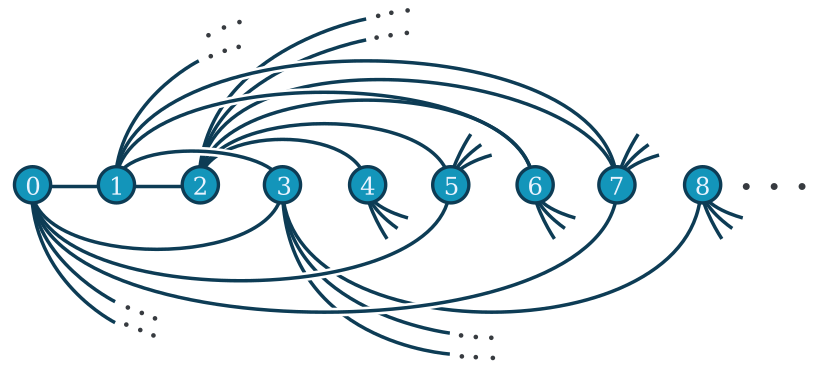
\includegraphics[scale=0.7]{Figures/Rado-graph.png}
	\caption{Binary construction of the Radó graph}
\end{figure}

\subsection{Erdös-Rényi model}
Erdös-Rényi model is the finite version of the Radó graph. In this model the parameter $p$ is usually taken as a function of $n$. This provide, unlike the past model, a variety of graphs even when $n$ tends to infinity.

\begin{defini}
Denote by $\G(n,p)$ to the probability space formed by all the graphs of $n$ vertices and probability measure 
$$ \P\Big(G\in \G(n,p)\Big) = p^{k} (1-p)^{\binom{n}{2}-k} $$
where $k$ is the number of edges in $G$, the $\sigma$-algebra is given by the power set.
\end{defini}

Note: There is a variation of the model, where we rather choose randomly exactly $m$ edges among the $\binom{n}{2}$ possible.

We can also think this model like $\binom{n}{2}$ i.i.d. $Bernoulli(p)$ that represent the edges. Using what we know about this r.v. we can immediately get some properties of the degree of a given vertex $v$.

\begin{itemize}
\item The probability that a given vertex $v$ has degree $k$ is given by
$$b(k; n-1,p) = \binom{n-1}{k} \cdot p^{k} \cdot (p-1)^{n-k-1}$$
\item The expected degree is $(n-1)\cdot p$
\item The variance of this degree is $(n-1)\cdot p \cdot (1-p)$
\end{itemize}

The degree distribution can be helpful to do optimizations in the rigid expansions algorithms. This is outlined in the next chapter.

\section{Rigid expansions}

 We will focus in the rigidity calculations for the finite case. Then, we will analyze when $n$ tends to infinite. For this, we need the calculations of the probability that the following events occur.

\begin{itemize}
\item A vertex $v$ is uniquely determined by $A_{m}$, a subset of vertices of size $m$
\item $A_k$ generate a rigid expansion
\item $A_k$ generate a rigid expansion with $s$ new elements
\end{itemize}

For the calculations concerning the first event, take a look to following picture

\begin{figure}[h!]
	\centering
	
\includegraphics[scale=1]{Figures/uni.png}
	\caption{Probability of uniquely determined vertices}
\end{figure}

If $<A_{m}> = v$, there is a edge between $v$ and every vertex in $A$, and none of the remaining $n-m-1$ vertices is also connected to every vertex in $A$, i.e.
$$\P (E_m) = \P(<A_{m}> = v) = p^{m}(1-p^{m})^{n-m-1}$$
Using the \texttt{networkx} library in \texttt{python} we reproduce the following experiment:

\begin{cajita}
\textbf{Uniquely determined vertex experiment} \hfill \break
Fixing $n,p,m$.
\begin{enumerate}
\item Generate an Erdös-Rényi graph $G\in \G(n,p)$ with labeled vertices.
\item Excluding the $n$-th vertex, take a random subset of vertices of size $m$.
\item Verify if this random set uniquely determine the $n$-th vertex.
\end{enumerate}
\end{cajita}

In the next chapter we explain how to generate random graphs for the first. To simplify the process we took, without loosing generality, the last vertex as a particular element of the experiment. When $m=n$ there is no need to do the experiment.

Fixing $n$ and $p$ we computed the empiric probability for each possible value of $m$. In the following figure appear these estimates together with the theoretical calculations.

\begin{figure}[h!]
	\centering
	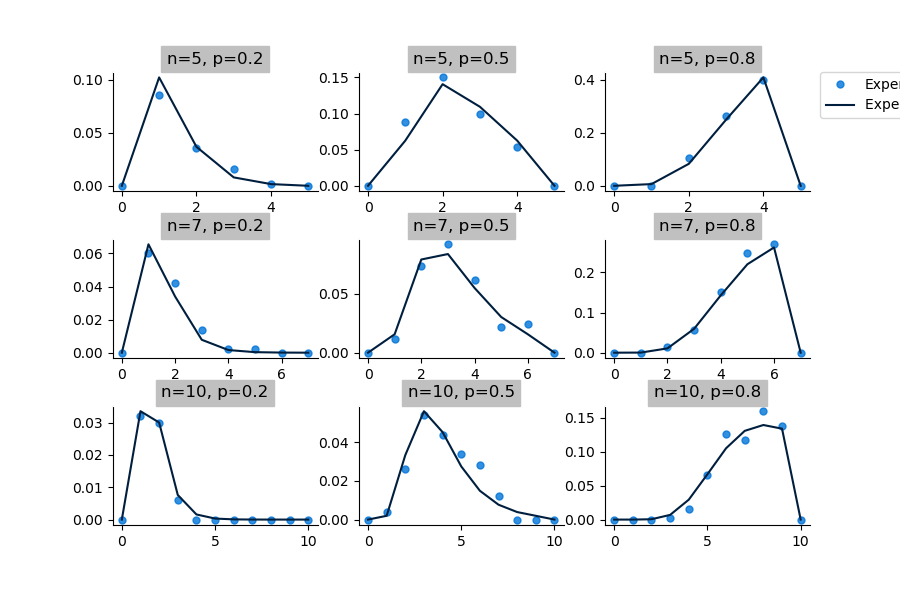
\includegraphics[scale=0.55]{Python/Figures/Uniquely-determinated-fixed-vertex.png}
	\caption{Theoretical and empirical probabilities of uniquely determined a vertex. For different values of $n$ and $p$ varying among all the possible values of $m$}
\end{figure}

For these calculations we repeated this experiment 500 times and count the number of times that the random set uniquely determine the $n$-th vertex. The empiric probability is the ratio of times when this happened.

Notice that there are certain values of $m$ more \textit{effective} than others, in the sense that, depending on the parameters of the model, it is more likely that a subset of certain size uniquely determine a vertex. This can be used, as described in the next chapter, to do optimizations in the simulations.
 
The following table is a summary of the maximum of differences between these two values for distinct values of $n$ and $p$. These values are indicators that the simulations and the calculations actually describe the same event.
\vspace{0.3cm}
\input{Python/Txt/Uniquely-determinated-fixed-vertex-table-errors.txt}
\vspace{-0.3cm}
 
For the second event, if $A_k$ does not generate a rigid expansion is because none of the subsets of $A_{k}$ determined uniquely a vertex outside of it. We have:
$$\P(A_k \text{ generates a rigid expansion}) = 1 -  \prod_{m=1}^{k} (\rho_{m,k})^{\binom{k}{m}}$$
where $\rho_{m,k} = \Big(1 -  \P(E_m)\Big)^{n-k}$.

Just as before, we reproduce the following experiment:
 
\begin{cajita}
\textbf{Rigid expansion experiment} \hfill \break
Fixing $n,p,k$.
\begin{enumerate}
\item Generate an Erdös-Rényi graph $G\in \G(n,p)$.
\item Take a random subset of vertices of size $k$.
\item Verify if this set generates a rigid expansion
\end{enumerate}
\end{cajita}

Notice that the third step is a critical point in this experiment; we must verify among all the possible subsets of $A_{k}$. In the next chapter we explain how this should be done.

Again, we repeated this experiment 500 times and calculated the empiric probability that a random set generate a rigid expansion. In the following figure appear empiric and theoretical probabilities for this experiment.

\begin{figure}[h!]
	\centering
	\includegraphics[scale=0.55]{Python/Figures/Expansion-probability-table-error.png}
	\caption{Theoretical and empirical probabilities of expanding $A_{k}$. For different values of $n$ and $p$ varying among all the possible values of $k$}
\end{figure}

The empirical and theoretical probabilities agree again.
\vspace{0.3cm}
\input{Python/Txt/Uniquely-determinated-fixed-vertex-table-errors.txt}
\vspace{-0.3cm}

The calculations for the last question are helpful if we want to approximate the sequence of rigid expansions of $A_{k}$ by a Markov chain. Consider $\{0,1, \dots n\}$ as the states space of the Markov chain with transition matrix given by:
$$ a_{k,k+s} = \P(A_{k} \text{ generates a rigid expansion by } s \text{ elements})$$
Notice that the deterministic process stops once a iteration fails to add new vertices. In our stochastic approximation a new $G \in \G(n,p)$ is considered for each step, hence, it is allowed to \textit{"have extra tries to expand".}

This probability calculations are more difficult to obtain. To start understanding this phenomenon we can simulate with our computational tools the following experiment:
 
\begin{cajita}                                                                                                                                                                
\textbf{Increase size by a rigid expansions experiment} \hfill \break
Fixing $n,p,k$.
\begin{enumerate}
\item Generate an Erdös-Rényi graph $G\in \G(n,p)$.
\item Take a random set of vertices $A_{k}$.
\item Produce the first rigid expansion from the graph spanned by $A_{k}$
\item Return the size of the expanded subgraph
\end{enumerate}
\end{cajita}

This experiment yields a random variable which depends on $n, p$ and $k$. Fixing $n$ and $p$ we obtained a sample of size 50 for every possible value of $k$. Using the resulting histogram as an empirical density function we obtain the following figure. It graphically describes the nature of the transition matrix of a sequence of rigid expansions.

\begin{figure}[h!]
	\centering
	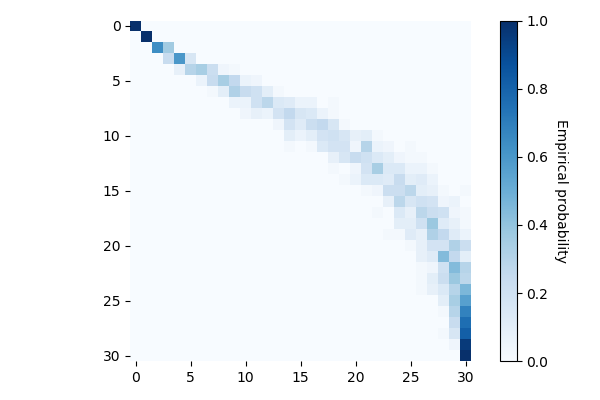
\includegraphics[scale=0.7]{Python/Figures/Transition-matrix-secuence-of-rigid-expansions.png}
	\caption{Empirical transition probability matrix}
\end{figure}

\section{Radó graph as a model for the curve graph}

In chapter one we settled the bases to model the curve graph associated to any given surface. Summarizing the results, the exposed models should, at least, guarantee the following properties:

\begin{enumerate}
\item Countably infinite number of vertices
\item Connectedness
\item Locally infinite
\item Clique number $3g-3+m$
\item Infinite diameter
\end{enumerate}

The Radó graph satisfy that every finite or countably infinite graph is an induced subgraph of it \cite{DarReferenciaAqui1}. The restriction in the clique number of $C(S)$ implies that, if $S$ is a surface of finite genus, is not possible that the Radó graph is embedded into $C(S)$. Even more, a result by by Bering and Gaster \cite{beringGaster} state that the converse is also valid.

\begin{theorem}
The random graph embeds into the curve graph $C(S)$ of a surface $S$ if and only if $S$ has infinite genus.
\end{theorem}

Therefore, if we want to study the curve graph of a surface of finite genus using the Radó graph, we have to think it as a subgraph of it. A simple but naive approach to do it is to take a random subset of vertices of a graph $G\in \G(\N, p)$ and then consider the vertex induced subgraph. It turns out that for a.e. $G\in \G(\N, p)$ the sequence $cl(G_n)$ is almost entirely determined.

\begin{theorem}
For a.e. $G \in \G(\N,p)$ there is a constant $m_0 = m_{0}(G)$ such that if $n \geq m_o$ and $n'_{r} \leq n \leq n_{r+1}$, then $cl(G_{n}) = r$.
\end{theorem}

The proof of this theorem can be find in \cite[Bollobás p.~284]{Bollobas}. The theorem states that if $r$ is fixed and finite, the number of vertices should be finite as well. Therefore, \textbf{it is not possible to obtain the curve graph by an uniform selection of vertices}. 

Notice that this property seems not generic at all, unlike the others listed above, the clique number is the only property which actually depends on the genus of the surface.

Complications like this appear often in the literature, for example in \cite{Alcazar15} they want to ensure that a random graph does not have cycles (in this case it is implied that the clique number is 2). A discrete MCMC algorithm was used to sample uniformly random trees of size $n$, with the \texttt{generate algorithm}. It produce a maximal tree of any not directed graph with $n$ vertices taken uniformly among all the possible ones. In the appendix we summarize the results of this method, for a deeper analysis look at \cite{Broder89}.

Even if we can provide an analog of the generate algorithm to ensure a fixed clique number, the idea is to study rigid expansions with a simpler probabilistic approach. In this spirit, it remains to examine the plausibility of the Erdös-Rényi model and do an asymptotic analysis.

\section{Erdös-Rényi as a model for the curve graph}

\subsection{Connectivity}
\begin{theorem}
Let $\omega(n)$ be a function that tends to infinity arbitrarily slow as $n$ tends to infinity
\begin{itemize}
\item If $p\geq \frac{log(n)+ \omega(n)}{n}$ then 
$$\lim_{n \to \infty} \P(G \in \G(n,p) \text{ is connected}) = 1$$
\item If $p\leq \frac{log(n)- \omega(n)}{n}$ then
$$\lim_{n \to \infty} \P(G \in \G(n,p) \text{ is disconnected}) = 1$$
\end{itemize}
\end{theorem}
 
This can be proven by first showing that for a large $n$ almost all graphs consists of a connected graph having $n-k$ effective vertices and $k$ isolated points, the theorem follows from a counting argument. The complete proof can be found in \cite[Erdös-Rényi, p. 59]{OnRandomGraphs}.
 
\subsection{Locally infinity}

The following theorem gives a complete description of the degree distribution; consider $X_{k} = X_{k} (G)$, the random variable that describes the number of vertices of degree $k$ in a graph $G$.

\begin{theorem}
Let $\epsilon>0$ be fixed, $\epsilon n^{-3/2} \leq p = p(n) \leq 1 - \epsilon n^{-3/2}$, let $k = k(n)$ be a natural number and set $\lambda_{k} = \lambda_{k}(n) = n\cdot b(k;n - 1,p)$. Then the following assertions hold.

\begin{itemize}
\item If $\lim \lambda_{k}(n) = 0$, then $\lim P(X_{k} = 0) = 1$. 
\item If $\lim \lambda_{k}(n) = \infty$, then $\lim P(X_{k} > t) = 1$
for every fixed $t$.
\item If $0 < \lim\lambda_{k}(n) < \lim \lambda_{k}(n) < \infty$,
then $X_{k}$ has asymptotically Poisson distribution with mean $\lambda_{k}$: 
$$P(X_{k} = r) \sim e^{\lambda_{k}}\cdot \lambda_{k}^{r}/ r!$$
for every fixed $r$.
\end{itemize}
\end{theorem}

The hypothesis on $p$ appears when we consider a loose upper bound on the expected degree of $X_ {k}$. If $pn^{2} \to \infty $ then almost every $ G \in \G (n, p) $ consist of independent edges and isolated vertices. The complete argument of this claim among with the proof of the theorem can be found in \cite[Bollobás, p.61]{Bollobas}.

If $k$ is a finite fixed number and $\lim \lambda_{k}(n) = 0$ then a.a.s there are no vertices of finite degree. In the second case there are an infinite number of vertices with degree $k$. In the third case we can describe explicitly the degree distribution, it will concentrated in a finite range around the mean $\lambda_{k}$. 

To ensure the locally infinite property using this theorem, $p = p(n)$ needs to satisfy the first case for any fixed $k$ i.e.
$$\lambda_{k} = n \binom{n-1}{k} p^{k} (1-p)^{n-k-1} \to 0$$
We can rather do a simplification of the matter using that $deg(v)$ behaves like a random binomial variable. Proposing a more simple expression for $p$ we can simplify the expressions which determine the threshold. 
\begin{theorem}\label{conectivityRCC}
Let $G \in \G(n,p)$, $\epsilon>0$ and $a>0$ be fixed, taking $p=\frac{\epsilon}{n^{a}}$ and 
\begin{itemize}
    \item If $a\geq 1$ then 
    $$\lim_{n \to \infty} \P(deg(v) \text{ is finite}) = 1$$
    \item If $a<1$ then
     $$\lim_{n \to \infty} \P(deg(v) \text{ is infinite}) = 1$$
\end{itemize}
\end{theorem}

\begin{proof}
We will assume that $a\neq 1$; when $a=1$ we know this is the Binomial's Poisson approximation. When $k=0$ we have
$$\displaystyle\lim_{n\to \infty} \P\Big(deg(v)= 0\Big) = \displaystyle\lim_{n\to \infty } \left( 1 - \frac{\epsilon}{n^a}\right)^n = \displaystyle\lim_{n\to \infty} exp\left( ln \left( 1 - \frac{\epsilon}{n^a}\right)^n\right) = \displaystyle\lim_{n\to \infty} exp\left(n \cdot ln \left( 1 - \frac{\epsilon}{n^a}\right)\right)$$
If $f(n)=  n \cdot ln \left( 1 - \frac{\epsilon}{n^a}\right)$, then $\displaystyle\lim_{n\to \infty} f(n) = \displaystyle\lim_{n\to \infty}\frac{ln \left( 1 - \frac{\epsilon}{n^a}\right)}{\frac{1}{n}}$. Using L'ôpital's rule for limits we obtain:
$$\displaystyle\lim_{n\to \infty } f(n) = 
\displaystyle\lim_{n\to \infty } \frac{\frac{1}{\left( 1 - \frac{\epsilon}{n^a}\right)}\cdot (\epsilon a n^{-a-1})}
{-1\cdot n^{-2}} = 
\displaystyle\lim_{n\to \infty } \frac{\frac{n^a}{n^{a} - \epsilon}\cdot (\epsilon a n^{-a-1}) \cdot {n^{2}}}{-1} = 
\displaystyle\lim_{n\to \infty } - \frac{\epsilon a n}{n^{a} - \epsilon} =
\displaystyle\lim_{n\to \infty } - \frac{\epsilon a}{a n^{a-1}}
$$
from here, if $a>1$ then $\displaystyle\lim_{n\to \infty } f(n) = 0$, if $a<1$ then $\displaystyle\lim_{n\to \infty } f(n) = -\infty$. So we have
$$ \displaystyle\lim_{n\to \infty} \P\Big(deg(v)=0\Big) = \begin{cases} 
\displaystyle\lim_{n\to \infty}e^{f(n)} = 1, & \mbox{if } a>1 \\ 
\displaystyle\lim_{n\to \infty}e^{f(n)} = 0, & \mbox{if } a<1 \end{cases} $$
Meaning that when $a>1$ then a.a.s the graph does not have any edges, this conclude the first part of the theorem. For $k>0$ and $a<1$:
\begin{center}
\begin{tabular}{ r l }
 $\displaystyle\lim_{n\to \infty } \P\Big(deg(v)=k\Big) =$ & $\displaystyle\lim_{n\to \infty} \binom{n}{k} \cdot \left( \frac{\epsilon}{n^a} \right)^k \cdot \left( 1-\frac{\epsilon}{n^a}\right)^{n-k}$ \\
$=$ &  $\displaystyle\lim_{n\to \infty} C_{k}\cdot n^k\cdot  \frac{\left(\frac{\epsilon}{n^a}\right)^k} {\left(\frac{n^a - \epsilon}{n^a}\right)^k} \cdot \left(1-\frac{\epsilon}{n^a}\right)^{n} $\\
$=$ &  $C_{k}\displaystyle\lim_{n\to \infty} n^k \cdot \left(\frac{1} {n^a - \epsilon}\right)^k \cdot \left(1-\frac{\epsilon}{n^a}\right)^{n} $\\
$=$ &  $C_{k} \displaystyle\lim_{n\to \infty}  n^s\cdot \left(1-\frac{\epsilon}{n^a}\right)^{n}$\\
\end{tabular}
\end{center}

where $s=k(1-a)>0$, hence $\displaystyle\lim_{n\to \infty } \P\Big(deg(v)=k\Big) = 0$

\end{proof}

\subsection{Clique number}

\begin{theorem}
Let $r = r(n) = O(n^{1/3})$ and let $p=p(n)$, $0<p<1$, be such that
$$\binom{n}{r} p^{\binom{r}{2}} \to \infty \text{ and } \binom{n}{r+1} p^{\binom{r+1}{2}} \to 0 $$
Then a.e $G\in\G(n,p)$ has clique number $r$.
\end{theorem}

The second condition on $p$ implies that almost no $G\in\G(n,p)$ contains a $K^{r+1}$ so $cl(G_{p})\leq r$ asymptotically almost surely. The first condition on $p$ is simply that $\E (X_{r}) \to  \infty$, where $X_r$ denote the random variable which counts the number of $r-$cliques in a graph $G$. This theorem can be proven using the calculations for $\E(X_{r})$ and a first moment argument. A full proof can be find in \cite[Bollobás, p.290]{Bollobas}.

Notice that in the hypothesis of the theorem $r$ is not fixed. Due that $r=3g-3+m$ this implies that the curve graph could corresponds to a surface whether of infinite diameter or with an infinite number of punctures

with the Stirling approximation for $\binom{n}{r}$ we can try to fit this result with the previous expressions.
$$E_{r} = (2\pi)^{- 1/2} n^{n+ 1/2} (n - r)^{-n+r-1/2} r^{-r-1/2} p^{r(r- 1)/2}$$
Taking $r$ as a fixed finite number we have
$$\displaystyle\lim_{n\to \infty } E_{r} = \displaystyle\lim_{n\to \infty} c_{r}\cdot \frac{n^{n+1/2}}{(n-r)^{n+1/2}} \cdot (n-r)^{r}\cdot p^{r(r-1)/2} = c_{r}\cdot \displaystyle\lim_{n\to \infty}  (n)^{r}\cdot p^{r(r-1)/2}$$
Taking $p=\epsilon/n^{a}$ as in \ref{conectivityRCC} it results in
$$\displaystyle\lim_{n\to \infty } E_{r} =  c_{r}\cdot \displaystyle\lim_{n\to \infty}  (n)^{r}\cdot\Big(\frac{1}{n^a}\Big)^{r/2}\cdo \Big(\frac{1}{n^a}\Big)^{r/2}
\cdot\frac{1}{n^a}$$



. Again, \textbf{this property interfere with the proposed model}. We can still provide an analogue of Bering and Gaster result.

\subsection{Diameter}

The diameter of a graph $G$, denoted by $diam(G)$, is the maximal distance between pairs of vertices of $G$.

For surfaces of finite genus we should had ensure infinite diameter. There are a number of theorems that state the conditions under this can be done \cite[Bollobás, p.259]{Bollobas}. Nevertheless, by the past results we must guarantee that the diameter is equal to 2, so the model match the properties of curve graphs for infinite genus surfaces.

\begin{theorem}
If $p$ is taken fixed $G(n,p)$ has diameter 2 with high probability 
\end{theorem}

\begin{proof}
Consider the random variable $X_{n}$ which is the number of vertex pairs in a graph in $\G(n,p)$ with no common neighbors. By Markov's inequality we have that
$$\P(X_{n} \geq 1)\leq \E(X_{n}) = \binom{n}{2} \cdot \P(\text{two vertices doesn't have common neighbors}) = \binom{n}{2} (1-p^{2})^{n-2}$$
which tends to zero as $n\to \infty$
\end{proof}

Although this result has a simple proof, the following theorem allows a broader type of functions to be taken, letting us refine the previous thresholds.

\begin{theorem}
Let $d$ be a fixed integer $d$, if 
$$\frac{(pn)^{d-1}}{n} \to 0 \text{ and } \frac{(pn)^{d}}{n} \to \infty $$
then, with probability approaching 1 as $n$ goes to infinity $G\in\G(n,p)$ has diameter $d$
\end{theorem}

The proof of this theorem is due to Klee and Larman and can be find in \cite{diameters}. For $d=2$ this mean that $p(n)= \frac{f(n)}{n^{1/2}}$ where $f(n)\in o(n^{1/2})$ and $f(n)\to \infty$.

Coupling with the expression for $p(n)$ in \ref{conectivityRCC}, this lead us to $a<\frac{1}{2}$



%In the first chapter we mention that 
%That's why it's worth to enunciate the following theorem which can be found in \cite[Khale, 16]{Khale}.
%\begin{theorem}
%Let $k \geq 3$ and $\epsilon > 0$ be fixed. If
%$$\left(\frac{(C_{k} + \epsilon \text{log } n} {n} \right) n^{1/k} \leq p \leq \frac{n^{-\epsilon}}{n^{1/(k+1)+\epsilon}}$$
%where $C_{3} = 3$ and $C_{k} = k/2 + 1$ for $k > 3$, then w.h.p. $X$ is rationally homotopy equivalent to a bouquet of $k$-dimensional spheres.
%\end{theorem}

%We can use the Erdös-Rényi model to obtain random simplicial complexes through clique complexes. The clique complex or flag complex $X(G)$, of a graph $G$ is the simplicial complex with all complete subgraphs of $G$ as its faces. The 1-skeleton of $X(G)$ is $G$ itself. $X(G(n, p))$ will be abbreviated by $X(n, p)$ for now on.
%The main remaining conjecture for the topology of random clique complexes is that these rational homotopy equivalences are actually homotopy equivalences.

%\begin{conje}
%The bouquet-of-spheres conjecture.
%Let $k \geq 3$ and $\epsilon > 0$ be fixed. If
%$$\frac{n^{\epsilon}}{n^{1/k}} \leq p \leq \frac{n^{-\epsilon}}{n^{1/(k+1)}}$$
%then w.h.p. $X$ is homotopy equivalent to a bouquet of $k$-spheres.
%\end{conje} 
% Chapter 3

\chapter{Computational experimentation} % Main chapter title

\label{Chapter3} % For referencing the chapter elsewhere, use \ref{Chapter1} 

\lhead{Chapter 3. \emph{Computational experimentation}} % This is for the header on each page - perhaps a shortened title

%----------------------------------------------------------------------------------------

Nowadays Scientific Computing is one the most important tools for Science. Computational implementation became crucial when the problem cannot be solved by traditional experimental or theoretical means. There are a number or reasons why this might happen, for example whenever experimentation may be dangerous, to expensive or time-consuming.

Stochastic topology has embraced the methods of scientific computing to provide a better insight of complex phenomena. For theoretical develop it has allowed, for example, to verify if the established conditions in a probabilistic model are sharp enough (\cite{Meshulam13}). 

Computational develop mixed with a strong probability background has demonstrated to be efficient and powerful. Algorithms based in random sampling has provided state-of-the-art techniques due to their great degree of flexibility and reliability.

The PageRank algorithm, was the first method used by Google to order search results \cite{pageRank}. It outputs a probability distribution used to represent the likelihood that a person randomly clicking on links will arrive at any particular page.

In motion planning, the use of Rapidly-exploring random trees (RRTs) are one of the most successful algorithms \cite{Alcazar15}. Problems in motion planning consist on finding a collision-free path that connects an initial configuration of geometric bodies to a final goal configuration. A RRT is a rooted tree that grows from a starting configuration by using random samples from the search space. 

In Bayesian Inference there is a family of algorithms, known collectively as Markov Chain Monte Carlo (MCMC), that allow us to approximate the posterior distribution as calculated by Bayes' Theorem.

In this chapter we use the outlined probabilistic material to accomplish an efficient implementation of rigidity phenomenon in graphs. This resulted in a computational tool that provide a richer insight of the concept. We describe our results with their technical difficulties and the actions taken to endure them.

All the computational experimentation was develop in \texttt{python}, it provide simple and flexible representations of networks as well as clear and concise expressions of network algorithms. The \texttt{\href{https://networkx.github.io/}{NetworkX}} library allowed to create and modify graphs as objects (dictionaries) and provided more features such as numerical linear algebra and drawing.

\section{Simulating Erdös-Rényi random graphs}

There is a direct algorithm to obtain a graph in $G(n,p)$, it simulate a $Bernoulli(p)$ r.v. for each of the $\frac{n(n-1)}{2}$ possible edges. Thus, it runs in $O(n^2)$ time. It is possible to do faster algorithms for small values of $p$ that runs in $O(n + m)$ time, where $m$ is the expected number of edges, which equals $\frac{pn(n - 1)}{2}$ \cite{fastER}.

In the figure \ref{fig:ErdosRenyi10} appears a set of graphs obtained with such algorithm, fixing $n=10$ an varying the parameter $p$.

\begin{figure}[h]
	\centering
	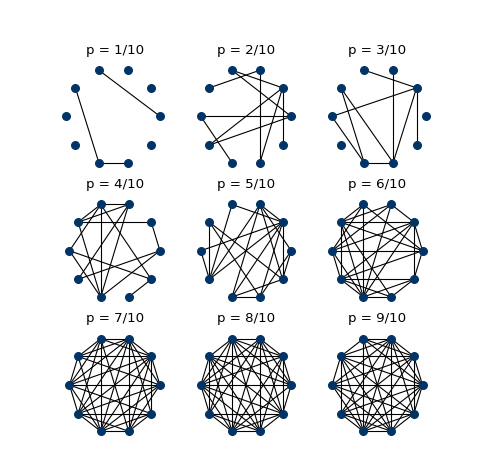
\includegraphics[scale=0.85]{Figures/ER-10.png}
	\caption{Erdös-Rényi random graphs with $n$ fixed and varying $p$}
	\label{fig:ErdosRenyi10}
\end{figure}

Figure \ref{fig:tiemposER} show the execution times varying $n$
\begin{figure}[h!]
	\centering
	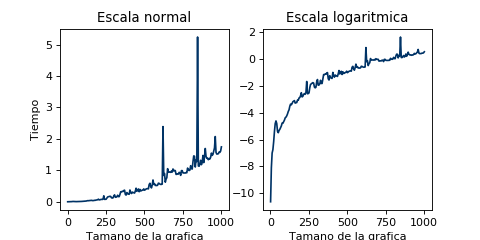
\includegraphics[scale=0.8]{Python/Figures/Times-ER.png}
	\caption{Execution times varying $n$. Both normal and logarithmic scale appear in the figure}
	\label{fig:tiemposER}
\end{figure}

\section{Rigid expansions algorithm}
A priory, the algorithm to determine a rigid expansion is supposed to be executed in a large amount of time. As the definition let us see, it depends on the size of $ G $, and it depends exponentially on the size of $A$; it must check among all the possible subsets of $A$, that is $2^{m}$ verifications, where $|A|=m$. Thus, it is important to do some optimization to the algorithms and evaluate when this have more impact in the expected execution time according to the parameters taken.

The following is the straightforward algorithm for rigid expansions.

\begin{cajita}
\textbf{Rigid Expansions Algorithm} \hfill \break

\begin{tabular}{ l l }
\texttt{Input:} &  \texttt{Random graph $G$ (dictionary),} \\
                &  \texttt{set of vertices $A$ (array).}\\
\texttt{Output:} & \texttt{Set of vertices obtained after expanding $A$ (array)} \\
\end{tabular}
\begin{enumerate}
\item Initialize N as empty (the set of new vertices)
\item For every $B$, subset of A:\hfill \break
\hphantom{12} If $\bigcap\limits_{b\in B} N(b) = v$ and $v\not\in A\cup N$: \hfill \break
\hphantom{1234} Add $v$ to $N$
\item If $N$ is not empty: \hfill \break
\hphantom{12} Replace $A$ by $A\cup N$ and return to step 1. \hfill \break
      Otherwise:\hfill \break
\hphantom{12} Return $A$
\end{enumerate}
\end{cajita}

In step two the iterations were indexed by \texttt{generators}. These are iterators in \texttt{python} were you can only iterate over once, so they do not store all the values in memory.

We proposed the following optimizations:

\begin{enumerate}
\item \textbf{Consideration of isolated vertices and leaves.} None of the isolated vertices in $A$ have any influence in rigid expansions, so they should not be consider. Also, whenever $A$ contains a leave is convenient to ignore them; the unique neighbor of a leave, which we will call \textit{petioles} should be automatically added in the first expansion an then it does not contribute in uniquely determine new vertices. This means that the input should be replace with:
$$A' = A - \{v: deg(v)\leq 1 \} \cup \{u: \exists x, N(x)=\{u\}\} $$
and add them again by the end of the expansions.
\item \textbf{Relative size of $A$.} In Step 2, if $A$ big enough is faster to check if a vertex outside of $A$ can be uniquely determinate by a subset of $A$. This can reduce dramatically the execution time when $p$ is small; it reduce the size of revisions by taking only the \textit{effective} part of $A$, this is convenient to do whenever
$$k\cdot log(2) > log(n-k) + (kp)\cdot log(2)$$
were $k$ is the size of $A$

\item \textbf{Restriction to effective subsets}. Calculations in Chapter 2 showed that there are subsets which are more likely to generate rigid expansions than others. This depend on the parameters of the space and the size of the subsets. If we restrict to these effective subsets we can reduce the number of verifications.
\end{enumerate}

With these optimizations we obtain the following algorithm

\begin{cajita}
\textbf{Optimized Rigid Expansions Algorithm} \hfill \break

\begin{tabular}{ l l }
\texttt{Input:} &  \texttt{Random graph $G$ (dictionary),} \\
                &  \texttt{set of vertices $A$ (array),} \\
                &  \texttt{$n$(int) and $p$(float)} \\
\texttt{Output:} & \texttt{Set of vertices obtained after expanding $A$ (array)} \\
\end{tabular}
\begin{enumerate}
\item Replace $A$ by $A'$
\item Initialize $N$ as petioles of $A$ (the set of new vertices)
\item Calculate the range of effective subsets.\hfill \break
If $k\cdot log(2) > log(n-k) + (kp)\cdot log(2)$: \hfill \break
\hphantom{12} For every $v\in V-A$:\hfill \break
\hphantom{1234} Take $C = A\cap N(v)$ and for every $B$, effective subset of C:\hfill \break
\hphantom{123456} If $\bigcap\limits_{b\in B} N(b) = v$ and $v\not\in A\cup N$: \hfill \break
\hphantom{12341234} Add $v$ to $N$

Otherwise:\hfill \break
\hphantom{12} For every $B$, effective subset of A:\hfill \break
\hphantom{1234} If $\bigcap\limits_{b\in B} N(b) = v$ and $v\not\in A\cup N$: \hfill \break
\hphantom{123456} Add $v$ to $N$

\item If $N$ is not empty: \hfill \break
\hphantom{12} Replace $A$ by $A\cup N$, initialize $N$ as empty and return to step 3. \hfill \break
      Otherwise:\hfill \break
\hphantom{12} Return $A\cup\{v: deg(v)\leq 1 \}$
\end{enumerate}
\end{cajita}

\section{Conclusions}

%Conclusiones sobre tu experimentación computacional.







%\input{./Chapters/Chapter4} 
%\input{./Chapters/Chapter5} 
%\input{./Chapters/Chapter6} 
%\input{./Chapters/Chapter7} 

%----------------------------------------------------------------------------------------
%	THESIS CONTENT - APPENDICES
%----------------------------------------------------------------------------------------

\addtocontents{toc}{\vspace{2em}} % Add a gap in the Contents, for aesthetics

\appendix % Cue to tell LaTeX that the following 'chapters' are Appendices

% Include the appendices of the thesis as separate files from the Appendices folder
% Uncomment the lines as you write the Appendices

% Appendix Template

\chapter{The generate algorithm} % Main appendix title

\label{AppendixA} % Change X to a consecutive letter; for referencing this appendix elsewhere, use \ref{AppendixX}

\lhead{Appendix A. \emph{The generate algorithm}} % Change X to a consecutive letter; this is for the header on each page - perhaps a shortened title

In this section we describe the algorithm due to \cite[Broder]{Broder89}. Given a not directed graph $G$ with $n$ vertices it produces a maximal tree of $G$ sampled uniformly among all the possibles. For almost every graph the expected executed time of the algorithm is $O(n\cdot log(n) )$ for each tree and O($n^{3}$) in the worst cases. 

One of the first algorithms published for this problem has execution time $O (n^{5})$. It is based on the fact that the total number of directed trees in a graph can be explicitly calculated through a determinant of $n \times n$ size. The algorithm consider the edges of the graph labeled from $1$ to $m$, each maximal tree is label by the set of its edges. This induces a lexicographic order in the set of trees and the same tree can be find calculation at most $m$ determinants. Further improvements by \cite{CDN88} and \cite{CDM88} reduce the number of calculations, thus reducing the execution time to $O(n^3)$ or $O(L(n))$, where $L(n)$ is the execution time of multiplying matrices of size $n\times n$, but the new algorithms turn out to be far more complicated.

For an stochastic approach, consider a particle that moves among vertices in a graph. At each step it moves, choosing uniformly random, from the current vertex to a neighbor of it. This stochastic process is a Markov chain called \textbf{Random Walk}.

\begin{cajita}
\textbf{Generate Algorithm}\hfill \break
\begin{tabular}{ l l }
\texttt{Input:} &  \texttt{Graph $G$ (dictionary),} \\
\texttt{Output:} & \texttt{Maximal tree $T$ (dictionary)} \\
\end{tabular}

\begin{enumerate}
\item Choose a random vertex $s$ of $G$ (uniformly).
\item Simulate a simple random walk in $G$. It stops when every vertex gets visited. 
\item For each $i$ in $V-s$ collect the edge $(j,i)$, the first entrance corresponds to the vertex where the particle was before it visited for the first time the vertex $i$. Let $T$ be the collection of such edges.
\item Return $T$.
\end{enumerate}
\end{cajita}

$T$ is a maximal tree because it contains $|V| - 1$ edges; it has an edge for every vertex in $G$ except for $s$, and by construction it does not contains cycles.

The \texttt{Generate} algorithm is based in a simulation of Markov chains in the space of interest. In this case, the Markov chain has a stationary distribution $\pi_{i}=d_{i}/\sum_{j\in V} d_{j}$ where $d_{i}$ is the degree of the vertex $i$. The pounded digraph associated to this chain $G_M =(V,E')$, is obtained by replacing each edge $\{i,j\}\in A$ by two directed edges; $(i,j)$ with weight $1/d_{i}$ and $(j,i)$ with weight $1/d_{j}$. The justification that the algorithm actually provides a method to sample with uniform distribution is summarized in the next three results, their proofs can be found in \cite{Broder89}.

Let $\mathcal{T}_{i}(G_{M})$ be the family of maximal directed trees of $G_{M}$ with root $i$, when the root is not under consideration it will be denoted simply by $\mathcal{T}(G_{M})$.

\begin{theorem}
Let $M$ be a irreducible Markov chain in $n$ states with stationary distribution $\pi_1, \dots, \pi_n$. Let $G_{M}$ be the weighted digraph associated to $M$. Then $$\pi_{i} = \frac{\sum_{ T \in \mathcal{T}_{i}(G_{M})} \omega (T)}{\sum _{T \in \mathcal{T}(G_{M})} \omega (T)}$$
where $\omega(T) = \prod_{a\in A(T)}\omega(a)$, this means that the weight of the a directed tree is defined as the product of the weight of the edges of the tree.
\end{theorem}

We define the (\textit{forward tree}) at time $t$, $F_{t}$ as follows: Let $I_{t}$ be the set of states visited before time $t+1$. For every $i\in I_{t}$, let $p(i,t)$ the first time that the state $i$ was visited. The root of the tree $F_{t}$ is $\{(X_{p(i,t)},X_{p(i,t)-1}) | i\in I_{t}-X_{0}\}$, where $(X_{t})_{t\in \N}$ corresponds to the Markov chain given by the random walk. In other words $F_{t}$ is constructed by overlapping the first entrance at each state with inverted orientation. Clearly $F_{t}$ is a directed tree with root where each edge points from the leaves to the root.

Let $C$ be the \textit{covering time}, i.e. the first time that all the states where visited. Clearly for $t\geq C$ the tree $F_{t}$ is a directed maximal tree and $F_{t}=F_{C}$. Note that with the past definition,the random walk $\{X_{t}\}$ in the vertices of $G_{M}$ induces a Markov chain $\{F_{t}\}$ in the space of all directed trees of $G_{M}$, it is called forward trees chain.

For this chain every no maximal tree is a transitive state and every maximal tree is an absorbent state. Even more, the next theorem establish the distribution of  $F_{C}$.

\begin{theorem}
With the same notation and conditions of the past theorem. Let $F_{C}$ be the forward tree in time $C$. Then, for any maximal directed tree with root $T$ of $G_{M}$ we have
$$\P(F_{C} = T) = \frac{\prod_{(i,j)\in T} P_{i,j}}{\sum_{T\in T(G_{M})} \prod_{(i,j)\in T'} P_{i,j}}$$
\end{theorem}

\begin{coro}
(Proof of the \texttt{Generate} algorithm) Let $M$ be a simple random walk in a connected non-directed graph $G = (V, E)$, staring from a vertex $s$, $G_{M}$ the directed graph associated to $M$ and covering time $C$ for $G$ starting from the stationary distribution, we have $F_{C}$ without considering direction is a maximal tree of $G$ with random uniform distribution among all the maximal possible trees of $G$.
\end{coro}

This algorithm can be implemented using \texttt{Python}. Fixing $G$ as the complete graph $K_{n}$ it was possible, using the generate algorithm, to sample uniformly from the set of maximal trees with $n$ vertices. In the figure \ref{fig:Arboles8} appear a set of trees obtained with this method, which are drawn using the function \texttt{draw$\_$random} of the \texttt{NetworX} library.

\begin{figure}[h!]
	\centering
	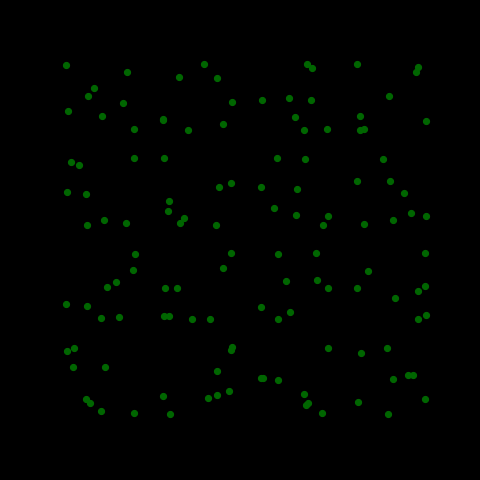
\includegraphics[scale=0.8]{Python/Figures/Arboles8.png}
	\caption{Maximal tree chosen randomly with uniform distribution among all the possible ones in complete graph (8) of vertices.}	
	\label{fig:Arboles8}
\end{figure}

The expected execution time of the algorithm per tree is equal to $\E(C_{s})$. It is known that for the connected graph $\E(C_{v}) = O(n^{3})$, nevertheless in \cite{BS89} there is a proof that if the transition matrix of a random walk have the second greater eigenvalue bounded away from 1, then the expected covering time is only $O(n\cdot log(n))$. Almost every graph in the Erdös-Rényi model satisfy his condition when $p > \frac{c\cdot log(n)}{n}$, in particular when $p=\frac{1}{2}$ and for almost every d-regular graphs \cite{BS87}, \cite{FKS89}. 
In the figure \ref{fig:tiemposGEN} appear the results of the execution time of the implemented algorithm.
\begin{figure}[h!]
	\centering
	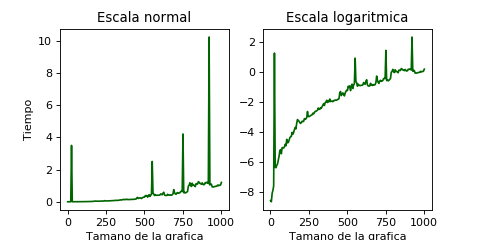
\includegraphics[scale=0.8]{Python/Figures/Time-generate.png}
	\caption{ Execution time of the algorithm in seconds varying the size of the tree. It appers the normal and the logarithmic scale}
	\label{fig:tiemposGEN}
\end{figure}

%\input{./Appendices/AppendixB}
%\input{./Appendices/AppendixC}

\addtocontents{toc}{\vspace{2em}} % Add a gap in the Contents, for aesthetics

\backmatter

%----------------------------------------------------------------------------------------
%	BIBLIOGRAPHY
%----------------------------------------------------------------------------------------

\label{Bibliography}

\lhead{\emph{Bibliography}} % Change the page header to say "Bibliography"

\bibliographystyle{ieeetr} % Use the "unsrtnat" BibTeX style for formatting the Bibliography

\bibliography{Bibliography} % The references (bibliography) information are stored in the file named "Bibliography.bib"




\end{document}